 
\documentclass[%
	%draft,
	%submission,
	%compressed,
	final,
	%
	%technote,
	%internal,
	%submitted,
	%inpress,
	reprint,
	%
	%titlepage,
	notitlepage,
	%anonymous,
	narroweqnarray,
	inline,
	twoside,
	invited
	]{ieee}

\usepackage[utf8]{inputenc}
\usepackage[spanish]{babel}
\usepackage{graphicx}
\usepackage{verbatim}
\usepackage{moreverb}
\usepackage{amsmath}
\usepackage{amsfonts}
\usepackage{amssymb}
\usepackage{fancybox}
\usepackage{float}
\usepackage{fancyvrb}
\usepackage{subfigure}

\newcommand{\latexiie}{\LaTeX2{\Large$_\varepsilon$}}

%\usepackage{ieeetsp}	% if you want the "trans. sig. pro." style
%\usepackage{ieeetc}	% if you want the "trans. comp." style
%\usepackage{ieeeimtc}	% if you want the IMTC conference style

% Use the `endfloat' package to move figures and tables to the end
% of the paper. Useful for `submission' mode.
%\usepackage {endfloat}

% Use the `times' package to use Helvetica and Times-Roman fonts
% instead of the standard Computer Modern fonts. Useful for the 
% IEEE Computer Society transactions.
%\usepackage{times}
% (Note: If you have the commercial package `mathtime,' (from 
% y&y (http://www.yandy.com), it is much better, but the `times' 
% package works too). So, if you have it...
%\usepackage {mathtime}

% for any plug-in code... insert it here. For example, the CDC style...
%\usepackage{ieeecdc}

\begin{document}

%----------------------------------------------------------------------
% Title Information, Abstract and Keywords
%----------------------------------------------------------------------
\title[Métodos de búsqueda no informados]{%
       Métodos de búsqueda no informados}

% format author this way for journal articles.
% MAKE SURE THERE ARE NO SPACES BEFORE A \member OR \authorinfo
% COMMAND (this also means `don't break the line before these
% commands).
\author[Castiglione, Karpovsky, Sturla]{Gonzalo V. Castiglione, Alan E. Karpovsky, Martín Sturla\\\textit{Estudiantes 
       Instituto Tecnológico de Buenos Aires (ITBA)}\\
\\\textbf{15 de Marzo de 2012}
}



\journal{Cátedra\ \ Sist.\ de\ Inteligencia\ Artificial,\ ITBA\ }
\titletext{-\ 15, MARZO\ 2012}
\ieeecopyright{\copyright\ 2011 ITBA}
\lognumber{}
\pubitemident{}
\loginfo{15 de Marzo, 2012.}
\firstpage{1}

\confplacedate{Buenos Aires, Argentina, 15 de Marzo, 2012}

\maketitle               

\begin{abstract} 
El presente informe busca analizar y comparar distintas estrategias de búsqueda no informadas sobre un problema en particular (Skyscraper puzzle) haciendo uso de un motor de inferencias.
\end{abstract}

\begin{keywords}
DFS, BFS, General Problem Solver, depth-first, breadth-first, search strategy
\end{keywords}

%----------------------------------------------------------------------
% SECTION I: Introduccion%----------------------------------------------------------------------
\section{Introducción}

\PARstart El juego \textit{Edificios} también conocido como \textit{Skyscraper puzzle} es una variante del conocido \textit{Sudoku} y consiste de una grilla cuadrada con números en su borde que representan las pistas sobre cuántos edificios se visualizan en esa dirección. El tablero, visto desde arriba, representa un espacio cubierto de edificios. Cada casillero debe ser completado con un dígito que va entre 1 y N, siendo N el tamaño de la grilla; haciendo que cada fila y cada columna contengan sólo una vez a cada dígito (como sucede en el Sudoku).

\par En este puzzle, cada dígito puesto en la grilla podría ser visualizado como un edificio de esa altura. Por ejemplo, si ingresamos un 5, estaríamos colocando un edificio de altura 5. Cada uno de los numeros que están por fuera de la grilla revelan la cantidad de edificios que pueden ser vistos al mirar la línea o columna en esa dirección. Cada edificio bloquea a todos los edificios de menor altura de ser vistos, mientras que los edificios de mayor altura son vistos a través de él.

%----------------------------------------------------------------------
% SECTION II: Marco Teórico
%----------------------------------------------------------------------

\section{Estados del problema}

\subsection{Estado inicial}

\par El estado inicial del problema es un tablero que contiene sólo las pistas en sus bordes (no contiene ningún edificio en la grilla). Para que el problema tenga solución éste tablero debe ser válido; es decir que no cualquier combinación de pistas sobre la visibilidad de edificios en esa dirección conducirán a un problema que resoluble.

\subsection{Estado final}

\par El estado final del problema es un tablero con todos los casilleros completos (lleno de edificios) que cumpla con las raglas del juego citadas anteriormente.

\section{Modelado del problema}

\par El tablero del juego se modeló mediante la creación de la clase Board; la misma contiene una variable privada de tipo matriz de enterios que representa a la grilla propiamente dicha. Si esta matriz es una determinada posición tiene un $0$, significa que ese casillero está vacío; si en cambio tiene un número $k \in [1,n]$ significa que allí hay situado un edificio con altura $k$.\\
\par Las pistas o restricciones del tablero (números en los bordes del mismo) las modelamos con arreglo de cuatro vectores de enteros (TOP, BOTTOM, LEFT, RIGHT) que simplemente contienen la restricción en esa dirección.\\

\begin{figure}[H]
\centering
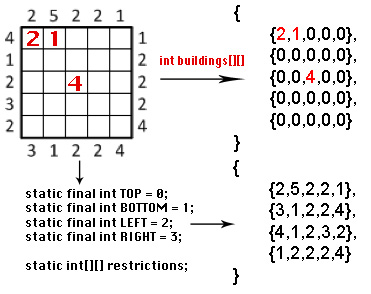
\includegraphics[scale=0.65]{./images/ModeladoSIA.jpg}
\caption{Modeladod el problema}
\label{modelado}
\end{figure}

\section{Reglas}

\par Dado un tablero de tamaño $n\times n$ podemos describir las reglas del problema en forma general como sigue:\\

\emph{Poner un edificio de altura $x$ en la posición $(i,j)$ del tablero, con $x \in [1, n]$.}\\

\par Por lo que, que dado un tablero de $n\times n$, el total de reglas está dado por $n \times {n \times n} = n^3$. Ya que, por cada fila, por cada columna, se tienen $n$ edificios distintos para colocar. 
\par Ejemplos de reglas:
\begin{itemize}
\item Poner un edificio de altura 1 en la posición $(0,0)$
\item Poner un edificio de altura 1 en la posición $(0,1)$
\item Poner un edificio de altura 2 en la posición $(0,0)$
\item Poner un edificio de altura 4 en la posición $(3,1)$
\item $\ldots$

\end{itemize}

\par Las reglas así definidas producen un factor de ramificación de $n^3$ lo que hace que, para tableros grandes (mayores a $5\times5$) se tarde un tiempo muy considerable en encontrar la solución. Para subsanar este inconveniente se puede planter el problema enunciando las reglas como siguen:\\

\emph{Poner un edificio de tamaño $a$ en el próximo lugar disponible de izquierda a derecha y de arriba hacia abajo.}\\

\par En nu tablero de $n\times n$ el conjunto de reglas quedaría definido de la siguiente forma:\\

\begin{itemize}
\item Poner un edificio de altura 1 en el próximo lugar disponible de izquierda a derecha y de arriba hacia abajo.
\item Poner un edificio de altura 2 en el próximo lugar disponible de izquierda a derecha y de arriba hacia abajo.
\item $\vdots$
\item Poner un edificio de altura $n$ en el próximo lugar disponible de izquierda a derecha y de arriba hacia abajo.
\end{itemize}

\par Esto nos otorga un factor de ramificación igual a $n$ siendo este muy inferior al del caso anterior. Si bien esta estrategia reduce la cantidad de reglas como así también el factor de ramificación, tomamos la decisión de implementar el primer conjunto de reglas [Poner un edificio de altura $x$ en la posición $(i,j)$] ya que, para la siguiente parte del TP, esto nos permitirá trabajar mejor con las heurísticas.



\subsection{Metareglas}

\par Si una restriccion (o pista) dice $n$ (siendo $n$ la dimensión del tablero) podemos definir una metaregla como sigue:\\

\emph{Colocar edificios de altura $1$ hasta $n$ en forma ordenada y ascendente en esa fila o columna}\\

\par Esto reduce considerablemente todos los algoritmos dado que quedarian menos casillas por explorar.

\section{Costos}

\par Debido a la naturaleza de nuestro probema, la aplciacion de todas las reglas tiene el mismo costo y éste es unitario. Es decir que la transición de un estado X a un estado Y, en nuestro caso, siempre nos cuesta $1$.

\section{Algoritmos de búsqueda implementados}

\par Hemos implementado cuatro algoritmos de búsqueda no informada diferentes. Los mismos son:

\begin{description}

\item[DFS]
Depth-first search

\item[BFS]
Breadth-first search

\item[IDFS]
Iterative DFS o profundización iterativa

\item[HIDFS]
Hybrid Iterative DFS

\end{description}

\section{Heurísticas}

\par La idea de las heurísticas, al tener un problema de satisfaccion de restricciones como el nuestro, no es hallar el camino óptimo a la solución ya que previamente sabemos su profundidad y su costo. Lo interesante de aplicar heurísticas en este caso es poder descartar caminos que no conducirán al algoritmo hacia la solución. Esto se logra, para un determinado nodo, asignándole el valor infinito a la función $h(n)$ de los sucesores irresolubles de éste.\\

\subsection{Heurística 1}
\par Dado un tablero de $n\times n$, si algunas de las restricciones contiene el número $n$, la fila o columna en esa dirección deberá contener los números de $1$ a $n$ en forma ordenada y ascendente.

\subsection{Heurística 2}

\par Si una restricción indica el número $1$, esa fila o columna deberá comenzar con la altura maxima $(n)$.

\subsection{Heurística 3}

\par Si una restricción indica algún número distinto de $1$ , esa fila o columna no podrá comenzar con $(n)$.

\subsection{Heurística 4}

\par Si una restricción indica algún número $a$ mayor o igual que $1$ , esa fila o columna deberá tener un edificio con la altura máxima $(n)$ a, al menos, $a$ casilleros de distancia. Esto es facil de ver ya que, considerando que ambos lados tienen restricciones (izquierda y derecha ó arriba y abajo), se puede localizar a algunos casilleros donde está la altura máxima. Por ejemplo, si tenemos $K$ como restricción izquierda y $R$ como restricción derecha, esto implica que la altura máxima tiene que estar a, al menos, $R$ casilleros desde la izquierda y a, al menos, $K$ casilleros desde la derecha.

\section{Resultados}


Estos resultados son consistentes con la siguiente tabla\footnote{Fierens, P. (2011), \emph{Cuadrados mínimos: repaso}, Buenos Aires: Instituto Tecnológico de Buenos Aires.}, la cual presenta el número de operaciones necesrias para resolver el problema de cuadrados mínimos cuando $A \in \Re ^{mxn}$:


\begin{table}[H]
\begin{center}
\begin{tabular}{|c|c|c|c|}
\hline
Algoritmo & Dimensión (n) & Tiempo & Nodos explotados\\
\hline
\hline

DFS & $2\times2$ & - & -\\
DFS & $3\times3$ & - & -\\
DFS & $4\times4$ & - & -\\
DFS & $5\times5$ & - & -\\
\hline
BFS & $2\times2$ & - & -\\
BFS & $3\times3$ & - & -\\
BFS & $4\times4$ & - & -\\
BFS & $5\times5$ & - & -\\
\hline
IDFS & $2\times2$ & - & -\\
IDFS & $3\times3$ & - & -\\
IDFS & $4\times4$ & - & -\\
IDFS & $5\times5$ & - & -\\
\hline
HIDFS & $2\times2$ & - & -\\
HIDFS & $3\times3$ & - & -\\
HIDFS & $4\times4$ & - & -\\
HIDFS & $5\times5$ & - & -\\

\hline  
\end{tabular}
\end{center}
\caption{Complejidad del problema de cuadrados mínimos}
\label{tmedio}
\end{table}

\section{Conclusión}

\PARstart Creemos que lorem ipsum dolor sit amet, consectetur adipisicing elit, sed do eiusmod tempor incididunt ut labore et dolore magna aliqua. Ut enim ad minim veniam, quis nostrud exercitation ullamco laboris nisi ut aliquip ex ea commodo consequat. Duis aute irure dolor in reprehenderit in voluptate velit esse cillum dolore eu fugiat nulla pariatur. Excepteur sint occaecat cupidatat non proident, sunt in culpa qui officia deserunt mollit anim id est laborum.


%----------------------------------------------------------------------
% The bibliography. This bibliography was generated using the following
% two lines:
%\bibliographystyle{IEEEbib}
%\bibliography{ieeecls}
% where, the contents of the ieeecls.bib file was:
%
%@book{lamport,
%        AUTHOR = "Leslie Lamport",
%         TITLE = "A Document Preparation System: {\LaTeX} User's Guide
%                  and Reference Manual",
%       EDITION = "Second",
%     PUBLISHER = "Addison-Wesley",
%       ADDRESS = "Reading, MA",
%          YEAR = 1994,
%          NOTE = "Be sure to get the updated version for \LaTeX2e!"
%}
%
%@book{goossens,
%        AUTHOR = "Michel Goossens and Frank Mittelbach and
%                  Alexander Samarin",
%         TITLE = "The {\LaTeX} Companion",
%     PUBLISHER = "Addison-Wesley",
%       ADDRESS = "Reading, MA",
%          YEAR = 1994,
%}
%
% The ieeecls.bbl file was manually included here to make the distribution
% of this paper easier. You need not do it for your own papers.

\clearpage

\begin{thebibliography}{1}

\bibitem{lamport1}
Fierens, P. (2011),
\newblock {\em Cuadrados mínimos: repaso},
\newblock Buenos Aires: Instituto Tecnológico de Buenos Aires.

\bibitem{lamport1}
Abdi, H.,
\newblock {\em  Least-squares: {Encyclopedia for research methods for the social sciences}},
\newblock Thousand Oaks (CA): Sage. pp, 2003.

\bibitem{lamport1}
Farebrother, R.W. (1988),
\newblock {\em Linear Least Squares Computations, STATISTICS: Textbooks and Monographs}, \newblock New York: Marcel Dekker.

\bibitem{lamport1}
Lipson, M.; Lipschutz, S. (2001),
\newblock {\em Schaum's outline of theory and problems of linear algebra}, 
\newblock New York: McGraw-Hill, pp. 69–80.


\end{thebibliography}

%----------------------------------------------------------------------


\clearpage

\onecolumn

\onecolumn
\section*{Anexo A: Gráficos ilustrativos}

\begin{figure}[H]
\centering
%\includegraphics[scale=0.7]{./images/ciudadRPTconajuste.png}
\caption{Curva que ajusta las velocidades medidas en la estación RPT, obtenida mediante eliminación gaussiana.}
\label{dataRPT}
\end{figure}

\begin{figure}[H]
\centering
%\includegraphics[scale=0.7]{./images/CIUDAD.PNG}
\caption{Error de la curva de ajuste obtenida por eliminación gaussiana, con respecto a las velocidades de la estación RPT.}
\label{dataRPT}
\end{figure}

\clearpage



\section*{Anexo B: Código}

\subsection{Código para la obtención de las matrices $A$ y $b$}

%\VerbatimInput{./code/calculoAb.m}




\end{document}
